\section{Decentralized Algorithm with Partial Information}
Generally speaking, the optimal policy could be obtained by solving the minimization problem on the right-hand-side of the above Bellman's equation. %Eqn. (\ref{eqn:sp_0}).
In our problem, however, the GSI is not available and the centralized agent design is impractical due to randomness of \brlatency.
On the other side, conventional value iteration algorithm is intractable due to the tremendous state space.
The number of system states and action space would grow exponentially with respect to the number of APs and edge servers.
In this section, we propose a low-complexity solution scheme where each AP updates its dispatching policy according to its OSI in an iterative manner.

\subsection{Low-Complexity Solution Framework}
The solution frame work is elaborated firstly in this subsection.

\comments{
    Due to the limit of OSI, each AP updates its policy independently from its corresponding ODI.
    Specifically, the $k$-th AP would update its policy once reception of the OSI, while considering other APs keep the policies fixed as the them in the OSI ($\forall k\in\apSet$).
    One AP updates the policy in one interval, while the other APs keep the policy fixed as broadcast information for the AP in updating.
    Hence we define the optimization problem for one AP as follows.
}

\begin{problem}[Decentralized Job Dispatching Problem]
    The disptaching optimization problem for the $k$-th AP ($\forall k\in\apSet$) is formulated, while the other APs follows the policy in the set $\set{ \mathcal{R}_{k'}(t) | \forall k'\in\ccSet_{k} }$ of $\Stat_{k}(t)$.
    \begin{align}
        \min_{\Omega_{k}} \lim_{T \to \infty}
            \mathbb{E}_{\Omega_{k}} \Bracket{
                \sum_{t=1}^{T} \gamma^{(t-1)} g_{k}\Paren{\Stat_{k}(t), \Omega_{k}(\Stat_{k}(t)) | \Stat_{k}(1)}
            },
    \end{align}
    where the \emph{system cost function} $g_{k}(\cdot)$ is define below.
    \begin{align}
        g_{k}\Paren{\Stat_{k}(t), \Omega_{k}(\Stat_{k}(t))} \define
            &\sum_{j\in\jSpace} \sum_{m\in\esSet_{\apSet}} \Brace{
                \Inorm{\vec{R}^{(k)}_{m,j}(t,0)}~+
                \nonumber\\
                &\{ Q_{m,j}(t,0) + \beta \cdot \mat{I}[Q_{m,j}(t,0)=L_{max}] \}
            }.
    \end{align}
    \label{problem_2}
\end{problem}
According to \cite{sutton1998introduction}, the above problem for the $k$-th AP could be solved by the following \emph{Bellman's equation}:
\begin{align}
    V_{k}\Paren{\Stat_{k}(t)} &= g_{k}\Paren{ \Stat_{k}(t) } + \gamma\min_{\Omega_{k}(\Stat_{k}(t))}
    \nonumber\\
    &\sum_{\Stat_{k}(t+1)} \Pr\Brace{ \Stat_{k}(t+1) | \Stat_{k}(t), \Omega_{k}(\Stat_{k}(t)) } \cdot V_{k}\Paren{\Stat_{k}(t+1)}.
    \label{eqn:sp_1}
\end{align}

\comments{
    In Eqn.(\ref{eqn:sp_1}), the transition function is not only determined by $\Omega_{k}(\Stat_{k}(t))$ but also the other APs' policy as part of OSI.
    Then, we update the individual policy of the $k$-th AP ($\forall k\in\apSet$) at one time in an iterative manner, where the policy adapted in the previous interval is taken as \emph{fixed policy} input of the next interval.
    % The $k$-th AP would be able to update its policy every $K$ broadcast interval for fairness.   
}
Specifically, we update the policy of each AP iteratively by solving the Problem \ref{problem_2}.
The details of the procedure is elaborated as follows.
\begin{itemize}
    \item Choose the initial \emph{system dispatching policy} start with some heuristic policy.
    \item At the first broadcast time slot when $t=0$, the APs and edge servers in \emph{conflict AP set} and \emph{candidate server set}, respectively, of the $1$-st AP would broadcast their LSI (including the heuristic policies);
    \item The $1$-st AP would receive the OSI at the $D_1(1)$ time slots in the first broadcast interval, and then it updates its policy $\Omega_{1}(\Stat_{1}(1))$ by solving Eqn.(\ref{eqn:sp_1}) for the $1$-st AP.
    The $1$-st AP would keep with this policy until it receives the OSI again.
    \item At the second broadcast time slot when $t=1$, the OSI of the $2$-nd AP would be broadcast;
    the $1$-st AP would broadcast $\Omega_{1}(\Stat_{1}(1))$ if it's in the \emph{conflict AP set} of the $2$-nd AP;
    \item Similarly, in the $t$-th broadcast interval the AP indexed with $k' \equiv (t + 1)\mod{K}$ would receive the OSI $D_{k'}(t)$ time slots later, and then it updates its policy $\Omega_{k'}(t+1)$ by solving Eqn.(\ref{eqn:sp_1}) for the $k'$-th AP.
\end{itemize}

However, solving Eqn.(\ref{eqn:sp_1}) with conventional value iteration algorithm is intractable due to the tremendous state space.
The number of system states and action space would grow exponentially with respect to the number of APs and edge servers.
In the following subsection, we will introduce a method to approximate the right-hand-side of the \emph{Bellman's equation} with one-step policy iteration.
%----------------------------------------------------------------------------------------%

\subsection{Value Function Analysis and Approximation}

In this subsection, we elaborate the method to approximate the Bellman's equation in Eqn.(\ref{eqn:sp_1}).

Firstly, we notice that the transition function in Eqn.(\ref{eqn:sp_1}) could be rewrite in the following form.
\begin{align}
    & \Pr\Brace{ \Stat_{k}(t+1)|\Stat_{k}(t), \Omega_{k}(\Stat_{k}(t)) }
    \nonumber\\
    =& \prod_{j\in\jSpace} \Brace{
        \prod_{k'\in\ccSet_{k}}\prod_{m\in\esSet_{k}} \Pr\big\{
            \vec{R}^{(k')}_{m,j}(t+1) | \vec{R}^{(k')}_{m,j}(t), \Omega_{k}(\Stat_{k}(t))
        \big\}
        \nonumber\\
        &\times \prod_{m\in\esSet_{k}} \Pr\big\{
            Q_{m,j}(t+1) | Q_{m,j}(t), \Omega_{k}(\Stat_{k}(t))
        \big\}
    },
\end{align}
where the transition function is decoupled into two parts of state transition on APs and edge servers, respectively.
To efficiently express the state transition, we further elaborate the distribution probability of the state vector as the corresponding probability vector, and perform the state transition with the transition matrix.

%NOTE: transition matrix and vector for AP
\begin{definition}[Denotation of Transition on AP]
    Let $\vecG{\Theta}^{(k)}_{m,j}(t,n)$ and ${\Gamma}^{(k)}_{m,j}(t,n)$ be the probability vector and transition matrix of $\vec{R}^{(k)}_{m,j}(t,n)$ at the $n$-th time slot in the $t$-th broadcast interval, respectively ($\forall k\in\apSet, m\in\esSet, j\in\jSpace$).
    \begin{align}
        \Gamma^{(k)}_{m,j}(t,n) &\define
        \begin{bmatrix}
            1 & \bar{p}^{(k)}_{m,j,0} &                       &        &                           \\
            & 0                     & \bar{p}^{(k)}_{m,j,1} &        &                           \\
            &                       & \ddots                & \ddots &                           \\
            &                       &                       & \ddots & \bar{p}^{(k)}_{m,j,\Xi-1} \\
            &                       &                       &        & 0                         \\
        \end{bmatrix},
        \\
        \vecG{\Theta}^{(k)}_{m,j}(t,n) &\define
        \Bracket{ \theta^{(k)}_{m,j,0}(t,n), \theta^{(k)}_{m,j,1}(t,n), \dots, \theta^{(k)}_{m,j,\Xi}(t,n) },
        % \begin{bmatrix}
        %     \theta^{(k)}_{m,j,0}(t,n) \\
        %     \theta^{(k)}_{m,j,1}(t,n) \\
        %     \vdots \\
        %     \vdots \\
        %     \theta^{(k)}_{m,j,\Xi}(t,n)
        % \end{bmatrix},
    \end{align}
    where $\theta^{(k)}_{m,j,\xi}(t,n)$ and $\bar{p}^{(k)}_{m,j,\xi}$ denote the probability of existing and offloading, respectively ($\forall \xi=0,\dots,\Xi$).
    \begin{align}
        \theta^{(k)}_{m,j,\xi}(t,n) &\define \Pr\{R^{(k)}_{m,j,\xi}(t,n) = 1\}
        \\
        p^{(k)}_{m,j,\xi} &\define \Pr\{U^{(k)}_{m,j} < (\xi+1) | U^{(k)}_{m,j}>\xi\}
        \\
        \bar{p}^{(k)}_{m,j,\xi} &= 1 - p^{(k)}_{m,j,\xi}.
    \end{align}
    And we note that $\theta^{(k)}_{m,j,0}(t,n)$ is purely determined by the arrival process and dispatching policy of the $j$-th type of job on the $k$-th AP, i.e. $\theta^{(k)}_{m,j,0}(t,n) = \lambda_{k,j} I[\omega_{k,j}(t,n) = m]$, where $I[\cdot]$ is the indicator function.

    Let $\hat{\vecG{\Theta}}^{(k)}_{m,j}(t)$ denote the probability vector at the first time slot of the $t$-th broadcast interval.
    Hence, the state transition between adjacent interval from $\hat{\vecG{\Theta}}^{(k)}_{m,j}(t+1)$ to $\hat{\vecG{\Theta}}^{(k)}_{m,j}(t)$ is composed of two-phase policy separated by $D_k(t)$, which could be expressed as follows.
    \begin{align}
        \vecG{\Theta}^{(k)}_{m,j}(t, \mathcal{D}_{k}(t)) &= (\Gamma^{(k)}_{m,j})^{\mathcal{D}_{k}(t)} \times \hat{\vecG{\Theta}}_{m,j}(t),
        \nonumber\\
        \hat{\vecG{\Theta}}^{(k)}_{m,j}(t+1) &= (\Gamma^{(k)}_{m,j})^{N-\mathcal{D}_{k}(t)} \times \vecG{\Theta}^{(k)}_{m,j}(t, \mathcal{D}_{k}(t)).
    \end{align}
\end{definition}

%NOTE: small probability approximation
% The expression of transition matrix $P_{m,j}$ is more complex.
The transition happening on edge servers is affect by the arrival process from APs.
Hence, we first denote the offloading matrix $\bar{\Gamma}^{(k)}_{m,j}$ from each AP to the $m$-th edge server and the offloading number vector $\vecG{\rho}^{(k,+)}_{m,j}({t,n})$ as follows, respectively ($\forall k\in\apSet, m\in\esSet_{m}, j\in\jSpace$).
\begin{align}
    \bar{\Gamma}^{(k)}_{m,j}(t,n) &\define
    \begin{bmatrix}
        0 & p^{(k)}_{m,j,0} &                 &        &                     \\
        & 0               & p^{(k)}_{m,j,1} &        &                     \\
        &                 & \ddots          & \ddots &                     \\
        &                 &                 & \ddots & p^{(k)}_{m,j,\Xi-1} \\
        &                 &                 &        & 1                   \\
    \end{bmatrix},
    \\
    \vecG{\rho}^{(k,+)}_{m,j}({t,n}) &\define \bar{\Gamma}^{(k)}_{m,j} \times \vecG{\theta}^{(k)}_{m,j}({t,n}).
\end{align}
The combinations of all the offloading number vector for the $m$-th edge server from its \emph{potential AP set} would be unacceptable.
Thus we rewrite the arrival process on edge server with small probability approximation, i.e. there would be at most one job arriving in one time slot, with the probability as the expected arrival rate of the original distribution.
The explicit definition of the approximate arriving probability $\beta_{m,j}({t,n})$ is given as follows.
\begin{align}
    {\beta}_{m,j}({t,n}) &\define \sum_{k\in\apSet} \sum_{\xi=0,\dots,\Xi-1} \mathbb{E}[\vecG{\rho}^{(k,+)}_{m,j,\xi}({t,n})]
    \label{eqn_0}
\end{align}
\begin{lemma}[Small Probability Approximation]
    The probability distribution of $\sum_{k\in\apSet} \vecG{\rho}^{(k,+)}_{m,j}({t,n})$ could be approximated with a Bernoulli arrival process who is with the expected arrival rate denoted as ${\beta}_{m,j}({t,n})$.
\end{lemma}
\begin{proof}
    \delete{v9}{
        We notice that the job arrival distribution ${\beta}_{m,j}(t)$ is given by $\mathcal{R}(t)$, and the departure rate in one slot is deterministic as $1/N$.
        Thus the expectation of ${\beta}$ would be always far more smaller than $1$ as composed of all $K$ AP nodes.
        We take approximation on ${\beta}$ as Bernoulli distribution in each time slot.
    }
\end{proof}

%NOTE: transition matrix and vector for Edge Server
Thus we could obtain the denotation of transition matrix and probability vector for edge servers.
\begin{definition}[Denotation of Transition on Edge Server]
    Let $\vecG{\mu}_{m,j}(t,n)$ and $P_{m,j}$ denote the probability vector and transition matrix of $Q_{m,j}(t,n)$ at the $n$-th time slot in the $t$-th broadcast interval, respectively ($\forall m\in\esSet, j\in\jSpace$).
    \begin{align}
        \vecG{\mu}_{m,j}(t,n) \define [\Pr\{Q_{m,j}=0\}, \dots, \Pr\{Q_{m,j}=L_{max}\}].
    \end{align}

    Let $\hat{\vecG{\nu}}_{m,j}(t)$ denote the probability vector at the first time slot of the $t$-th broadcast interval.
    The time-variant transition matrix composed of multiple transition matrix $P_{m,j}(\beta({t,n}))$ in all the time slots in $i$-th interval as follows.
    \begin{align}
        \vecG{\nu}({t,n+1}) &= P_{m,j}\Paren{\beta_{m,j}({t,n})} \vecG{\nu}({t,n})
        % \label{eqn_3}
        \\
        \hat{\vecG{\nu}}(t+1) &= \prod_{n=0,\dots,N-1} P_{m,j}\Paren{\beta_{m,j}({t,n})} \hat{\vecG{\nu}}(t),
        \label{eqn_4}
    \end{align}
\end{definition}

According to the additive structure of cost function, we substitute the transition function plus value function in Eqn. (\ref{eqn:sp_1}) under some \emph{fixed policy} $\Pi_{k}$ with two linearly sections as $W^{\AP}_{\Pi_{k}}(\mathcal{R}(t+1))$ and $W^{\ES}_{\Pi_{k}}(\mathcal{Q}(t+1))$ for APs and edge servers, respectively.
\begin{definition}[Low-complexity Bellman's Euqation]
    \begin{align}
        V_{k}(\Stat_{k}(t)) = g_{k}(\Stat_{k}(t)) + \gamma \min_{\Baseline_{k}} \Bracket{
            W^{\AP}_{\Pi_{k}}\Paren{\mathcal{R}(t+1)} + W^{\ES}_{\Pi_{k}}\Paren{\mathcal{Q}(t+1)}
        },
        % &V_{k}(\Stat_{k}(t)) = g_{k}(\Stat_{k}(t)) +
        % \nonumber\\
        % &~~~~~~\gamma \min_{\Baseline(t)} \Bracket{ W^{\AP}_{\Baseline(t)}\Paren{\mathcal{R}(t+1)} + W^{\ES}_{\Baseline(t)}\Paren{\mathcal{Q}(t+1)} },
    \end{align}
    where $W^{\AP}_{\Pi_{k}}(\cdot)$ and $W^{\ES}_{\Pi_{k}}(\cdot)$ are defined as follows, respectively.
    \begin{align}
        W^{\AP}_{\Pi_{k}}\Paren{\mathcal{R}(t)}
            &\define \sum_{j\in\jSpace}\sum_{k'\in\ccSet_{k}}\sum_{m\in\esSet_{k}}
            \nonumber\\
            &\mathbb{E}_{\{\Baseline(t), \vec{R}^{(k')}_{m,j}(t)\}}\Bracket{
                \sum_{i=0}^{\infty} \gamma^{i} \Inorm{\vec{R}^{(k')}_{m,j}({t+i})}
            }
        \\
        W^{\ES}_{\Pi_{k}}\Paren{\mathcal{Q}(t)}
            &\define \sum_{j\in\jSpace}\sum_{m\in\esSet_{k}}
            % \nonumber\\
            \mathbb{E}_{\{\Pi_{k}, Q_{m,j}(t)\}}\Bracket{
                \sum_{i=0}^{\infty} \gamma^{i} Q_{m,j}({t+i})
            }.
    \end{align}
\end{definition}
Hence, the optimization problem \ref{problem_2} could be further simplified with a efficient form.

%----------------------------------------------------------------------------------------%
\subsection{The Decentralized Optimization Problem}
In this subsection, we formulate the optimization problem with approximated Bellman's equation, which could solve Eqn.(\ref{eqn:sp_1}) more efficiently with analytical performance guarantee.
% The optimization problem at right-hand side of approximate Bellman's Equation is given as follows.
\begin{problem}[Decentralized Approximated Optimization Problem]
    The problem \ref{problem_2} is reduced to the following form under \emph{fixed policy} $\Pi_{k}$ for the $k$-th AP.
    \begin{align}
        \min_{\Pi_{k}} W^{\AP}_{\Pi_{k}}\Paren{\mathcal{R}(t+1)} + W^{\ES}_{\Pi_{k}}\Paren{\mathcal{Q}(t+1)}.
        \label{eqn:partial}
    \end{align}
\end{problem}

The expected value function $W^{\AP}_{\Pi_{k}}(\mathcal{R}(t+1))$ is easily obtained by calculating the following equation.
\begin{align}
    W^{\AP}_{\Pi_{k}}\Paren{\mathcal{R}(t+1)} = \sum_{j\in\jSpace}&\sum_{k\in\ccSet_{k}}\sum_{m\in\esSet_{k}}
    \nonumber\\
    &\Inorm{
        \Paren{ 1 - \gamma ({\Gamma}^{(k)}_{m,j})^{N} }^{-1} \hat{\vecG{\Theta}}^{(k)}_{m,j}(t+1)
    }.
    \label{w_ap}
\end{align}
% where $\hat{\Gamma}^{(k)}_{m,j} \define (\Gamma^{(k)}_{m,j})^{N}$.

The expression for expected value function $W^{\ES}_{\Pi_{k}}(\mathcal{Q}(t+1))$ is little more complex compared to Eqn.(\ref{w_ap}).
It is affected with both arrival process under dispatching policy and last queue state.
However, we notice that the arrival process would be stationary after the maximum uploading time under the stationary baseline policy and the relationship between APs and edge server could be decoupled.
\begin{align}
    W^{(k)}_{\Baseline(t)}\Paren{\mathcal{Q}(t+1)}
    =& \sum_{j\in\jSpace}\sum_{m\in\esSet_{k}}\sum_{i=0,\dots,\frac{\Xi}{T}} \gamma^{i} \mathbb{E}[ Q_{m,j}({t+i+1}) ]
    \nonumber\\
    &~~~~~~~~+ \gamma^{\frac{\Xi}{T}} \Paren{ \mat{I} - \gamma \hat{\mat{P}}_{m,j}(\tilde{\beta}_{m,j}) }^{-1} \vecG{\nu}({t+\frac{\Xi}{T}+1}) \vec{g}',
\end{align}
where the $i$-th element of vector $\vec{g}$ denotes the cost of server as $Q_{m,j}(t)$;
\begin{align}
    \hat{\mat{P}}_{m,j}(\tilde{\beta}_{m,j}) \define \prod_{n=0,\dots,N-1} \mat{P}_{m,j}(\tilde{\beta}_{m,j})
\end{align}
% the probability distribution of $Q_{m,j}({t+i+1})$ is denoted by $\vecG{\nu}({t+i+1})$ which is obtained by calculating equation Enq. (\ref{eqn_0}) - Eqn. (\ref{eqn_4}) ($\forall i=0,\dots,\frac{\Xi}{T}$);
where $\tilde{\beta}_{m,j}$ is the arrival distribution under baseline policy $\Pi(t)$ (on $m$-th ES with $j$-type job)
\begin{align}
    \tilde{\beta}_{m,j} &\define \sum_{k\in\apSet} \tilde{\lambda}^{(k)}_{m,j} \times \sum_{\xi=0,\dots,\Xi-1} \Pr\{ \xi<U_{k,m}\leq(\xi+1) \}
        \nonumber\\
    ~~~~&= \sum_{k\in\apSet} \tilde{\lambda}^{(k)}_{m,j}
\end{align}

\begin{lemma}
    The optimized policy solved as $\Baseline(t)$ for next stage, is better than $\Baseline(t-1), \dots, \Baseline(1)$ when considering the \emph{approximated value function} defined above.
    \\
    Moreover, the performance of the series of the baseline policies is upper bounded by the optimal solution $\Policy^*$ when considering the original Bellman's equation.
    $$
        V_{\Omega^*}\Paren{\Stat(t)}
        \leq W_{\Baseline(t)}\Paren{\Stat(t)}
        \leq W_{\Baseline(t-1)}\Paren{\Stat(t)}
        % \leq \dots \leq W_{\Pi(1)}\Paren{\Stat(t)}
    $$
\end{lemma}
\begin{proof}
    The proof is delete.
\end{proof}
%----------------------------------------------------------------------------------------%
\delete{v8}{
    We introduce a heuristic dispatching algorithm as the baseline policy, whose value function could be derived analytically.
    Then the right-hand-side of Bellman's Equation is replaced with the above approximated Bellman's equation, and the sub-optimal solution can be obtained with one-step policy iteration.
    Hence, the derived approximated value function of the baseline policy becomes the cost upper bound of the proposed sub-optimal policy.

    Moreover, we remove the assumption on centralized agent in the problem formulation by using partial information observed from each AP, and APs iteratively apply policy update.
    Under this scheme, we could further reduce the state information required for one AP and alleviate the impact of \brlatency.
    Then we leverage the sub-optimal solution obtained above, and replace the expression with reduced state information.
}

\delete{v9}{
    % \begin{figure}[htp!]
    %     \centering
    %     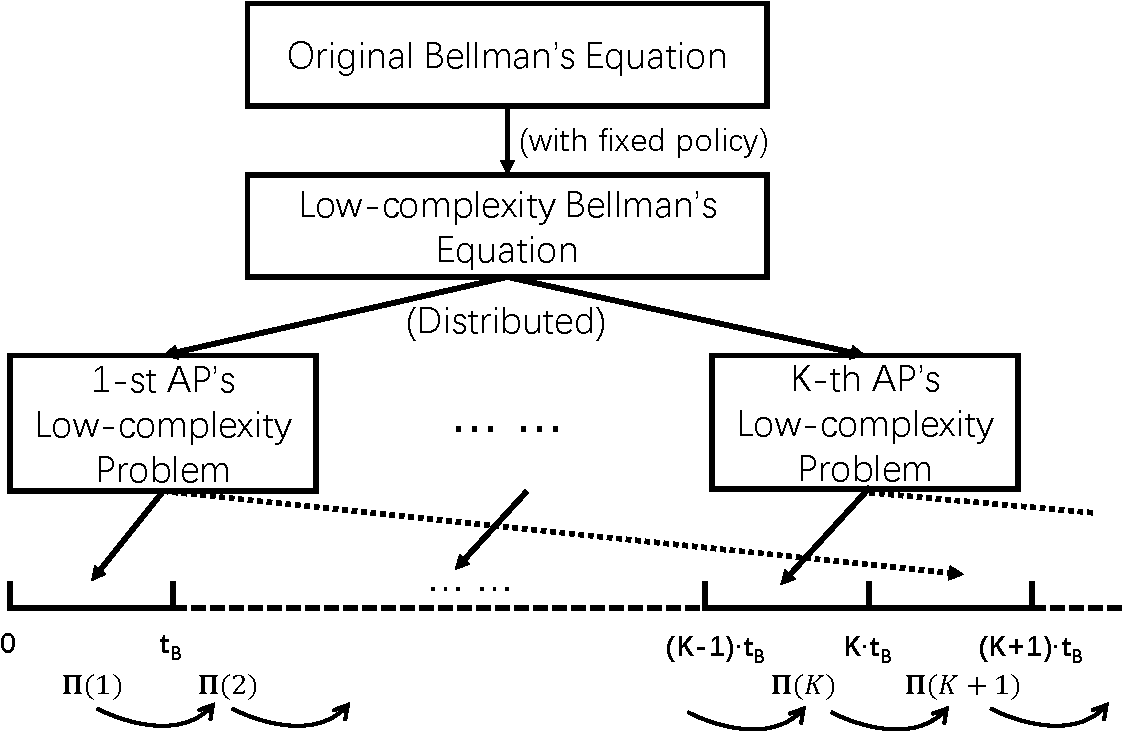
\includegraphics[width=0.45\textwidth]{images/solution-framework.pdf}
    %     \caption{The illustration of how low-complexity solution framework works over timeline.}
    %     \label{fig:solution}
    % \end{figure}
    % The whole picture of our low-complexity solution scheme is depicted in Fig.\ref{fig:solution}.

    % We use the same baseline policy to evaluate both low-complexity policy performance in Eqn. (\ref{eqn:sp_0}).
    % To better analyze the structure of the optimization problem, we decouple the transition function.

    % [\IF, \ENDIF], [\FOR, \TO, \ENDFOR], [\WHILE, \ENDWHILE], \STATE, \AND, \TRUE
    % \begin{algorithm}[H]
    %     \caption{Online Iterative Policy Improvement Algorithm}
    %     \begin{algorithmic}[1]
    %         \STATE $t = 0$
    %         \FOR{$t = 1,2,\dots$}
    %             \STATE Evaluate $\Omega_0$ in \textbf{P1} according to Eqn. (\ref{sp1})
    %             \FOR{$k \in \mathcal{K}$}
    %                 \STATE fix policy $\vec{\Omega}^{(k)}(t) \forall k' < k$
    %                 \STATE Evaluate $k$-th AP Local Policy $\tilde{\Omega}_k$ in \textbf{Pk} according to Eqn. (\ref{sp2})
    %             \ENDFOR
    %         \ENDFOR
    %     \end{algorithmic}
    % \end{algorithm}
}
%----------------------------------------------------------------------------------------%